
\documentclass[compress]{beamer}

%\usepackage{beamerthemesplit}
\usepackage{xmpmulti}


\usepackage{multirow}
\usepackage{multicol}
\usepackage{booktabs}
\usepackage{graphicx,float,wrapfig, bbm}
\usepackage{amsfonts, bbold, comment}
\usepackage{mdwlist}
\usepackage{subfigure}
\usepackage{colortbl}
\usepackage{overpic}
\usepackage{pdfpages}

\usepackage{multirow}

\pgfdeclareimage[width=\paperwidth]{mybackground}{../../common/boulder.pdf}

\newcommand{\name}[0]{\textsc{caco}}
\newcommand{\vect}[1]{\bm{\mathbf{#1}}}
\newcommand{\slda}[0]{\abr{slda}}
\newcommand{\bm}[1]{\mbox{\boldmath$#1$}}
\newcommand{\lda}[0]{\abr{lda}}
\newcommand{\explain}[2]{\underbrace{#2}_{\mbox{\footnotesize{#1}}}}
\newcommand{\itmspace}[0]{\hspace{2cm}}
\newcommand{\pos}[1]{{\texttt{#1}}}
\newcommand{\e}[2]{\mathbb{E}_{#1}\left[ #2 \right] }
\newcommand{\ind}[1]{\mathbb{I}\left[ #1 \right] }
\newcommand{\abr}[1]{\textsc{#1} }
\newcommand{\ex}[1]{\mbox{exp}\left\{ #1\right\} }
\newcommand{\h}[2]{\mathbb{H}_{#1}\left[ #2 \right] }
\newcommand{\g}{\, | \,}
\newcommand{\popshow}[2]{\only<#1->{\alert<#1>{#2}}}
\newcommand{\citename}[1]{#1 }
\newcommand{\flag}[1]{{\setlength{\fboxsep}{0pt}\fbox{\includegraphics[height=0.30cm,width=0.45cm]{clwe/flags/#1.pdf}}}}

\newcommand{\fsi}[2]{
\begin{frame}[plain]
\vspace*{-1pt}
\makebox[\linewidth]{\includegraphics[width=\paperwidth]{#1}}
\begin{center}
#2
\end{center}
\end{frame}
}


\newcommand{\danquote}[1]{

\begin{flushright}
\begin{overpic}[width=5.5cm,tics=10]{general_figures/speech_bubble}
	\put(10,30) { \parbox{4cm}{#1 }}
\end{overpic}

\includegraphics[width=1.5cm]{general_figures/milkman_dan}
\end{flushright}
}


\newcommand{\gfxi}[2]{
\begin{center}
	\includegraphics[width=#2\linewidth]{interpretability/#1}
\end{center}
}

\newcommand{\gfxs}[2]{
\begin{center}
	\includegraphics[width=#2\linewidth]{simtrans/#1}
\end{center}
}

\newcommand{\gfxq}[2]{
\begin{center}
	\includegraphics[width=#2\linewidth]{qb/#1}
\end{center}
}


\newif\ifjobtalk\jobtalktrue
\newif\iflong\longtrue

\usetheme[
          showdate=true,                     % show the date on the title page
          alternativetitlepage=true,         % Use the fancy title page.
          titlepagelogo=general_figures/shell,              % Logo for the fir\
st page.
          ]{UMD}


\title[]{Multilingual Situation Frame Prediction}
\author{Jordan Boyd-Graber, Benjamin Van Durme, Philip Resnik, Ting
  Hua, \dots}
\date{GRACE BBN: UMD / JHU / CU}

\institute[] % (optional, but mostly needed)
{University of Maryland}


%gets rid of bottom navigation symbols
\setbeamertemplate{navigation symbols}{}

%gets rid of footer
%will override 'frame number' instruction above
%comment out to revert to previous/default definitions
\setbeamertemplate{footline}{}

\begin{document}

\frame{
\titlepage
\tiny
}


\begin{frame}{Recap: How we're doing SF}

  \begin{itemize}
    \item Cross-lingual word embeddings (CLWE) \popshow{2}{(Bad, OOV words)}
    \item Use both translation and original text \popshow{2}{(MT makes mistakes)}
    \item Bag of words model \popshow{2}{(Why not sequence?)}
  \end{itemize}

\end{frame}

\begin{frame}{Three Issues}

\begin{enumerate}
  \item How do we know if cross-lingual embeddings are any good?
  \item Why don't sequence models degrade well with noisy MT input?
  \item How can we deal with OOV input words?
\end{enumerate}

\end{frame}

\begin{frame}{Question 1: What makes a good embedding}

  \begin{itemize}
    \item Dictionary translations should have high \emph{cosine
        similarity}
    \item QVEC  (Tsvetkov et al., 2015)
      \begin{itemize}
        \item Correlation of linguisticly-derived vector with word
          dimension
        \item Higher correlation better
      \end{itemize}
     \pause
     \item But both of these require extensive resources
     \item Can we do something simple?
  \end{itemize}

\end{frame}

\begin{frame}{Look at nearest neighbor graph}

  \begin{itemize}
    \item Form a graph of each words $k$ nearest neighbors
    \item Look at the language of the nearest neighbors
      \begin{itemize}
        \item Languages in their own neighborhood: bad
        \item Mixed languages: good
          \pause
        \item Modularity
       \end{itemize}

  \end{itemize}

\end{frame}

\fsi{clwe/uighur_modularity}{Unmixed word embeddings}

\begin{frame}{Modularity}

Given $L$ different languages, modularity $Q$ is defined as:
\begin{equation}
\label{unnorm_modularity}
Q = \sum_{l = 1}^L (e_{ll} - a_l^2),
\end{equation}
where $e_{ll}$ is the fraction of edges that are connected to the same language:
\begin{equation}
e_{ll} = \frac{1}{2m} \sum_{ij} A_{ij} \delta(g_i=l) \delta(g_j=l),
\end{equation}
and $a_{l}$ is the expected fraction of edges connected to the same language:
\begin{equation}
a_{l} = \frac{1}{2m} \sum_{i} d_{i} \delta(g_i=l),
\end{equation}
where $m$ is the number of edges and $\delta$ is an indicator function that evaluates to $1$ if the argument is true and $0$ otherwise.

\end{frame}

\begin{frame}{Predicting Classification Accuracy}

\begin{columns}
  \column{.4\linewidth}
  Predict classification {\bf excluding}:
  \begin{itemize}
    \item \alert<3>{Modularity}
    \item \alert<2>{QVEC}
    \item \alert<1>{Cosine}
  \end{itemize}
  \column{.6\linewidth}
  \begin{center}
    \only<3->{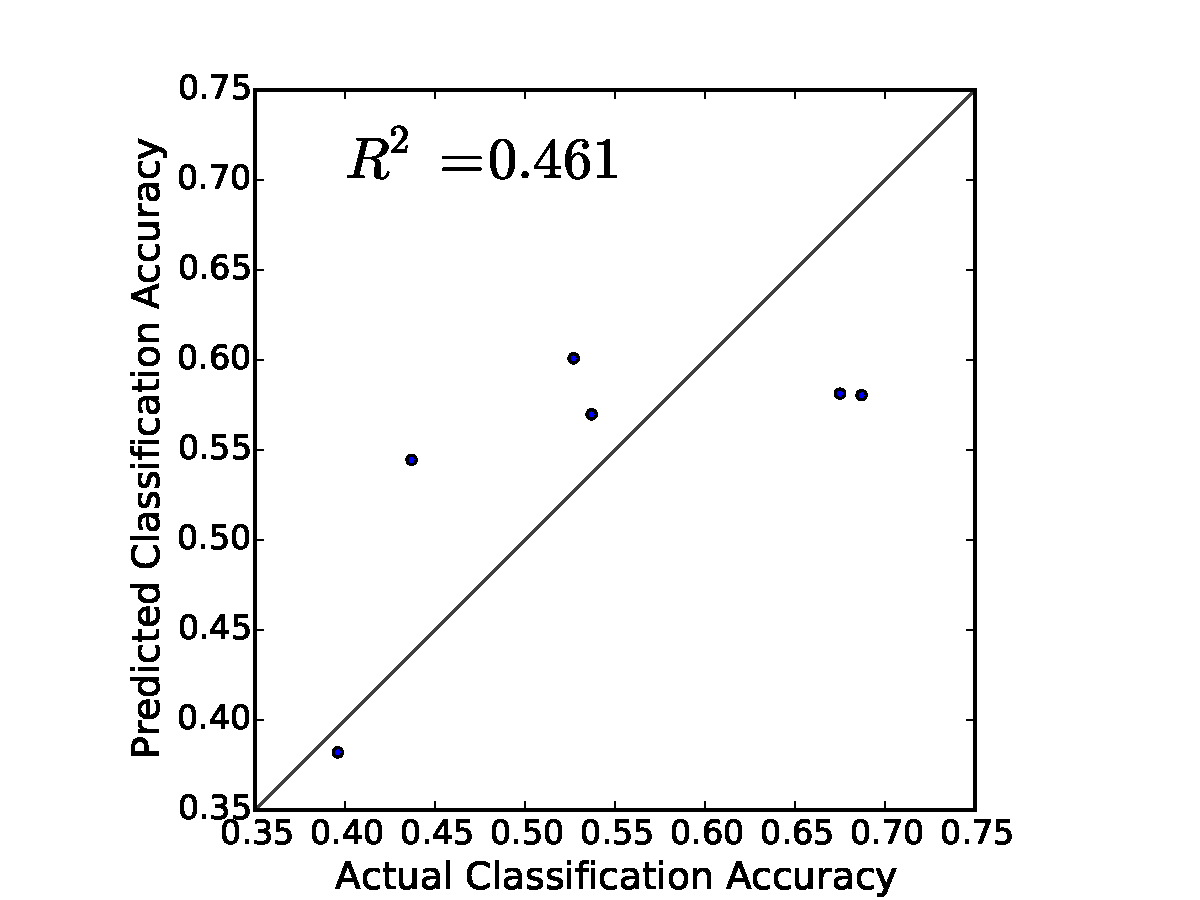
\includegraphics[width=.9\linewidth]{clwe/0_ablated}}
    \only<2>{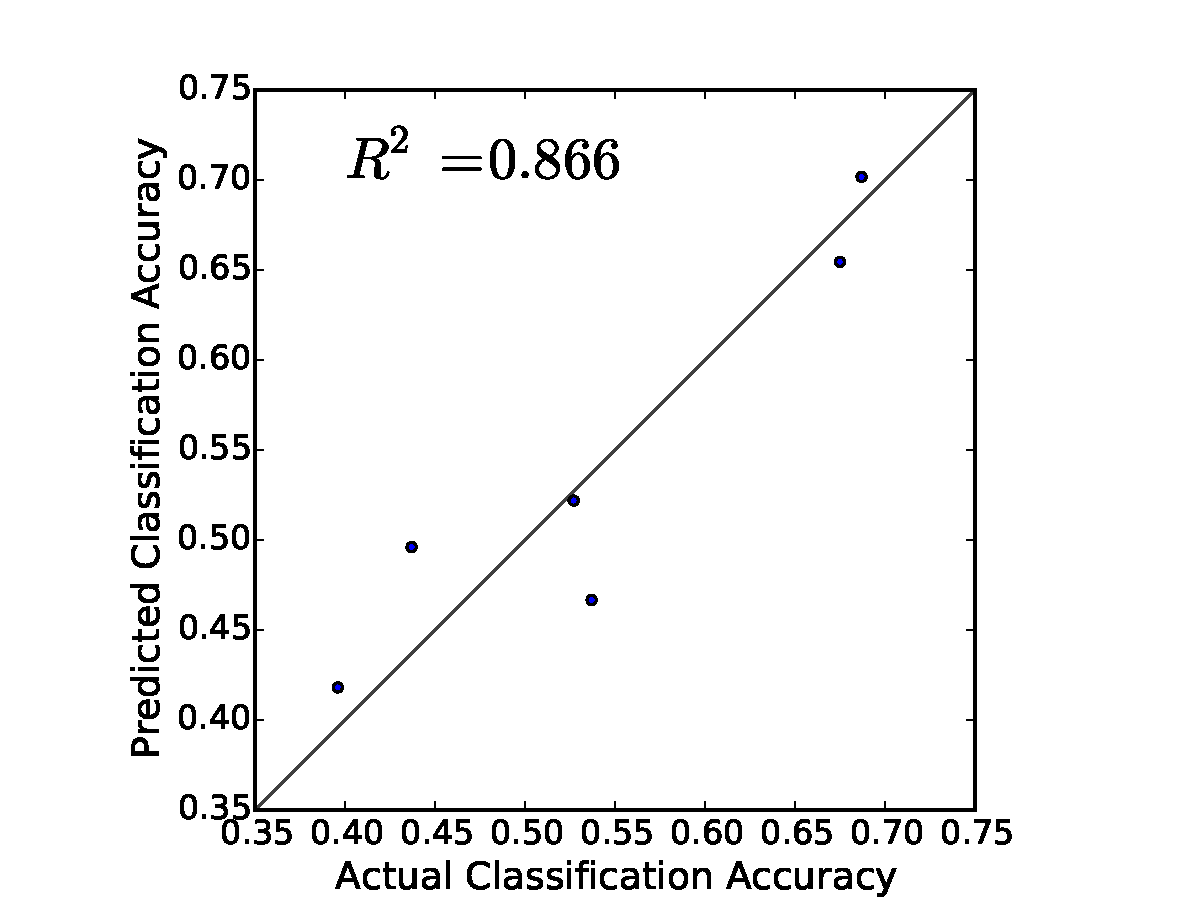
\includegraphics[width=.9\linewidth]{clwe/1_ablated}}
    \only<1>{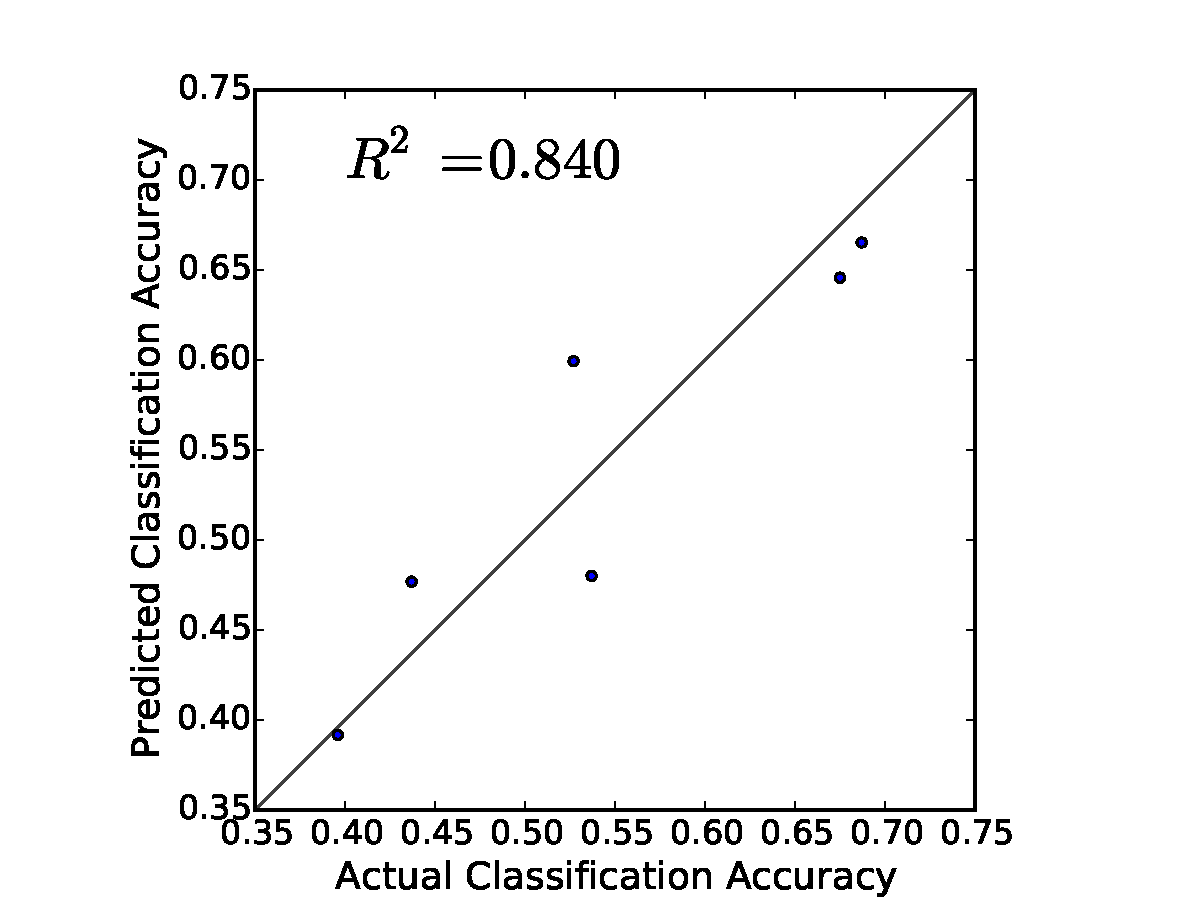
\includegraphics[width=.9\linewidth]{clwe/2_ablated}}
  \end{center}
\end{columns}
\vspace{1cm}
\only<4>{Takeaway: modularity works well without huge resources}

\end{frame}

\begin{frame}{Next steps}

  \begin{itemize}
    \item We can tell bad from good, but unclear if helpful for good
      vs. great
    \item How to extend to many languages at once
    \item How to know when to trust \emph{specific} word embeddings
  \end{itemize}

\end{frame}

\begin{frame}{Question 2: Why Do Sequence Models Degrade Poorly?}

\begin{itemize}
  \item We train models on perfect, complete English data
  \item But at test time, we have problems
    \begin{itemize}
      \item Translation errors
      \item OOV words
      \item Hard to predict problems in advance
    \end{itemize}
  \item Not much luck with sequence models on SF task
\end{itemize}

\end{frame}

\begin{frame}{Crazy things can happen}
  Let's start removing words from examples and see what happens when
  applying RNN model to tiny example \dots
  \begin{itemize}
    \item Situation frame: ``during'' $\rightarrow$ {\bf Terrorism}
      \pause
    \item Sentiment: ``must'' $\rightarrow$ {\bf Positive}
      \pause
    \item Question Answering \dots
  \end{itemize}

  \end{frame}

\fsi{rawr/heat_map_1}{All these questions get answer right}

\begin{frame}{RAWR}
  \begin{itemize}
    \item Can get really short while giving same answer
      \begin{center}
        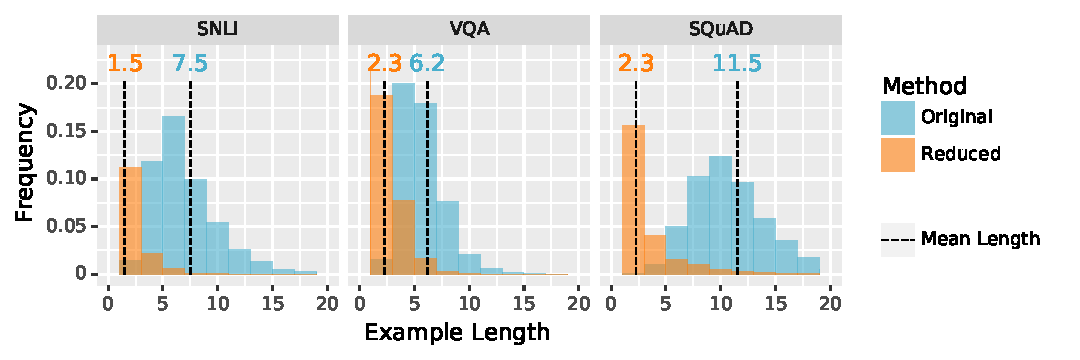
\includegraphics[width=.9\linewidth]{rawr/length_histogram}
      \end{center}
    \item We call these examples ``Right Answer, Wrong Reason''
    \item Not all of these are reasonable decisions
  \end{itemize}

\end{frame}

\begin{frame}{Fixing the problem}

  \begin{itemize}
    \item Training on full sentences leads to unexpected behavior on
      shorter inputs
    \item Solution: add entropy regularizer to emphasize
      \emph{uncertainty}
      \begin{equation*}
      \sum_{(x, y) \in (X, Y)}\log(f(y \g x)) + \lambda\sum_{\tilde{x}\in \tilde{X}}
       \h{}{f(\cdot \g \tilde{x})}.
    \end{equation*}
  \end{itemize}

\end{frame}

\begin{frame}{Improves raw performance and robustness}

\begin{itemize}
  \item On most languages and tasks, RNN performance goes up .5 to 1.0
    $f$-measure
  \item Requires longer example to trigger (double the length)
  \pause
\item Bag of word models still do
better on SF
\begin{itemize}
  \item Too little data?
  \item Syntax irregular / unimportant?
\end{itemize}

\end{itemize}


\end{frame}

\begin{frame}{Question 3: Dealing with OOV Words}
  \begin{columns}
    \column{.5\linewidth}
    \begin{center}
      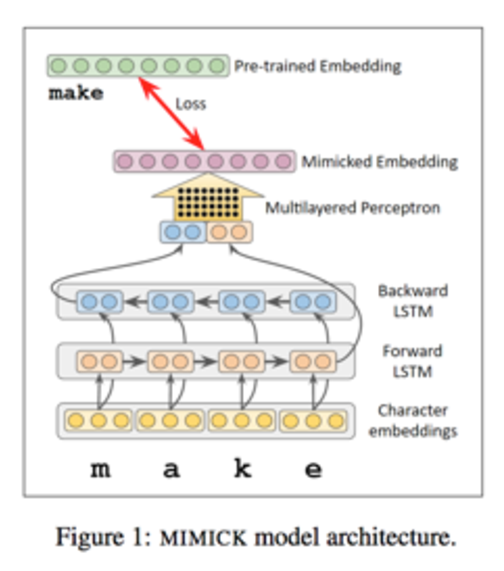
\includegraphics[width=.9\linewidth]{clwe/mimick}
    \end{center}
    \column{.5\linewidth}
  \begin{itemize}
    \item Hacky solution: use MIMICK (Pinter et al, 2017)
      \begin{itemize}
        \item Train on Amharic characters
        \item Apply to Tigrinya
          \begin{center}
            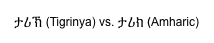
\includegraphics[width=.9\linewidth]{clwe/amharic}
          \end{center}
      \end{itemize}
    \item Can we do better with full model?
  \end{itemize}
  \end{columns}
\end{frame}

\fsi{clwe/architecture}{Embedder (LSTM) feeds into classifier (DAN)}

\begin{frame}{Objective}

  \begin{itemize}
    \item Classifier accuracy (source language)
\begin{equation}
    L_s(\theta) = -\frac{1}{|S|}\sum_{\langle \vect{w}, y \rangle \in S}
    \log p(y \mid \vect{w}; \theta),
\end{equation}
    \item Get things in dictionary right
      \begin{equation}
        L_d(\theta) = \frac{1}{|D|}\sum_{\langle w, w' \rangle \in D}
        ||e(w) - e(w')||_2^2.
      \end{equation}
      \item Use pre-trained embeddings if you have / trust them
        \begin{equation}
          L_e(\theta) = \frac{1}{V} \sum_{i=1}^V ||e(w_i) - x_i||_2^2
        \end{equation}
        \item Complete objective
         \begin{equation}
  L(\theta) = \explain{classifier}{L_s(\theta)} + \lambda_d \explain{dictionary}{L_d(\theta)} + \lambda_e \explain{embed}{L_e(\theta)},
\end{equation}
  \end{itemize}

\end{frame}

\begin{frame}{Character Transfer Results}

  \begin{itemize}
    \item Sanity check: compare with MIMICK hack
      \begin{itemize}
        \item Improvement on IL5 (+0.1)
        \item Drop on IL6 (-0.2)
      \end{itemize}
      \pause
      \item Roughly doing what we had before
      \item Fuller model allows more exploration
      \item Other annotations
  \end{itemize}

\end{frame}

\begin{frame}{Experiment Setup}

\begin{itemize}

\item Cross-lingual document classification (CLDC) experiments on RCV2 (Klementiev et al., 2012).
\item Two North Germanic and three Romance languages.
\item Word-based models: DAN with 40-dim multiCCA/multiCluster CLWE (Ammar et al., 2016).
\item {\bf C}lassification {\bf A}ided by {\bf C}onvergent {\bf
O}rthography (CACO) variants:
\begin{itemize}
\item SRC: labeled data only
\item DICT: labeled data + dictionary matching
\item MIM: labeled data + mimicking
\item ALL: everything
\item DICT+, ALL+: variants with language identifiers.
\end{itemize}

\end{itemize}

\end{frame}

\begin{frame}{Character Transfer Results}
\tiny
\begin{table}
  \centering
  \begin{tabular}{ll|rr|rrrrrrr}
    & & \multicolumn{2}{c|}{word-baed \abr{dan}} & \multicolumn{6}{c}{\name{} variants}\\
    source & target & multiCCA & multiCluster & \abr{src} & \abr{dict} & \abr{dict+} & \abr{mim} & \abr{all} & \abr{all+}\\
    \hline
    \flag{da}~\abr{da} & \flag{sv}~\abr{sv} & 67.5 & 58.5 & 51.0 & 60.5 & 53.5 & 66.0 & \textbf{69.5} & 68.0\\
    \flag{sv}~\abr{sv} & \flag{da}~\abr{da} & 51.0 & 36.0 & 52.0 & \textbf{70.5} & 46.5 & 63.0 & 59.5 & 55.0\\
    \flag{es}~\abr{es} & \flag{fr}~\abr{fr} & \textbf{60.0} & 37.0 & 47.0 & 51.0 & 48.5 & 51.5 & 48.5 & 48.5\\
    \flag{es}~\abr{es} & \flag{it}~\abr{it} & 54.0 & 55.0 & 49.0 & 50.0 & 47.0 & 46.5 & \textbf{59.0} & 44.5\\
    \flag{fr}~\abr{fr} & \flag{es}~\abr{es} & 61.0 & \textbf{65.5} & 62.5 & 60.5 & 65.0 & 58.0 & 60.0 & 54.0\\
    \flag{fr}~\abr{fr} & \flag{it}~\abr{it} & 46.0 & \textbf{64.5} & 46.5 & 43.5 & 57.0 & 48.5 & 53.5 & 47.0\\
    \flag{it}~\abr{it} & \flag{es}~\abr{es} & 42.5 & 42.0 & 54.5 & \textbf{62.0} & 54.5 & 58.0 & 45.5 & 47.5\\
    \flag{it}~\abr{it} & \flag{fr}~\abr{fr} & 26.5 & \textbf{59.5} & 42.5 & 56.5 & 52.0 & 46.5 & 56.0 & 50.5\\
    \hline
    \multicolumn{2}{r|}{average} & 51.1 & 52.3 & 50.6 & \textbf{56.8} & 53.0 & 54.8 & 56.4 & 51.9\\
  \end{tabular}
  \caption{\label{tab:result} Results of \abr{cldc} experiments on eight
  related language pairs from Reuters RCV2.  The best result for each row is in
  \textbf{boldface}.  The \name{} models are competitive with \abr{clwe}-based
  \abr{dan} models that use far more resources.}
\end{table}


\end{frame}

\begin{frame}{Challenges}
    \begin{itemize}
    \item Doesn't always work (Romance to Germanic)
    \item What about different scripts?  (Uighur and Tajik)
    \item Using multiple languages at once
      \pause
    \item Annotation remains bottleneck
   \end{itemize}
  \end{frame}


\begin{frame}{Wrapup}

  \begin{itemize}
    \item We need good CLWE models; how can we diagnose
    \item Sequence models are brittle
    \item Transferring information between languages
      \pause
      \item Other things we're thinking about
    \begin{itemize}
      \item Harvesting / annotation data
      \item Using spatial-temporal domain
      \item Corpus-level interactions with NI
    \end{itemize}
  \end{itemize}

\end{frame}

\fsi{clwe/il5_med}{IL5: Medicine}

\fsi{clwe/il6_regime}{IL6: Regime}

\end{document}
